\section{2D System Simulation}

\subsection{System overview}
The system presented is a Multiple Input Multiple Output (MIMO) system, such that in this case there are 4 inputs and 2 outputs. 

The 2 outputs that it is needed to control are:
\begin{itemize}
	\item Drone's antenna angle ($\theta_{d}$)
	\item Groundstation's antenna angle ($\theta_{gs}$)
\end{itemize}

The system's inputs are as follows:
\begin{itemize}
	\item Drone's antenna angle ($\theta_{d}$)
	\item Groundstation's antenna angle ($\theta_{gs}$)
	\item Drone position ($x_{drone},y_{drone}$)
	\item Groundstation position ($x_{gs},y_{gs}$)
\end{itemize}

\begin{figure}
	\centering
	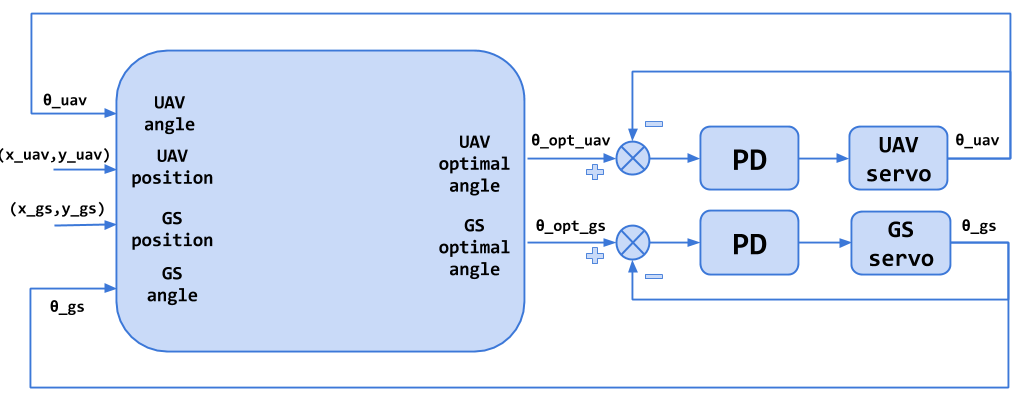
\includegraphics[scale=0.42]{figures/2d_system.png}
	\caption{2D sytem overview}
	\label{fig:2d_system}
\end{figure}

\subsection{Optimal Angle}
The first block of the system takes as inputs the parameters above and computes the optimal angles for the ground station ($\theta_{opt_gs}$) and drone ($\theta_{opt_d}$) antennas, such that a strong communication link is achieved.  


\subsection{Scenario}
In Figure \ref{fig:drone_gs} it is shown a scenario where the antennas of both GS and drone change after some periods of time.

\begin{figure}
	\centering
	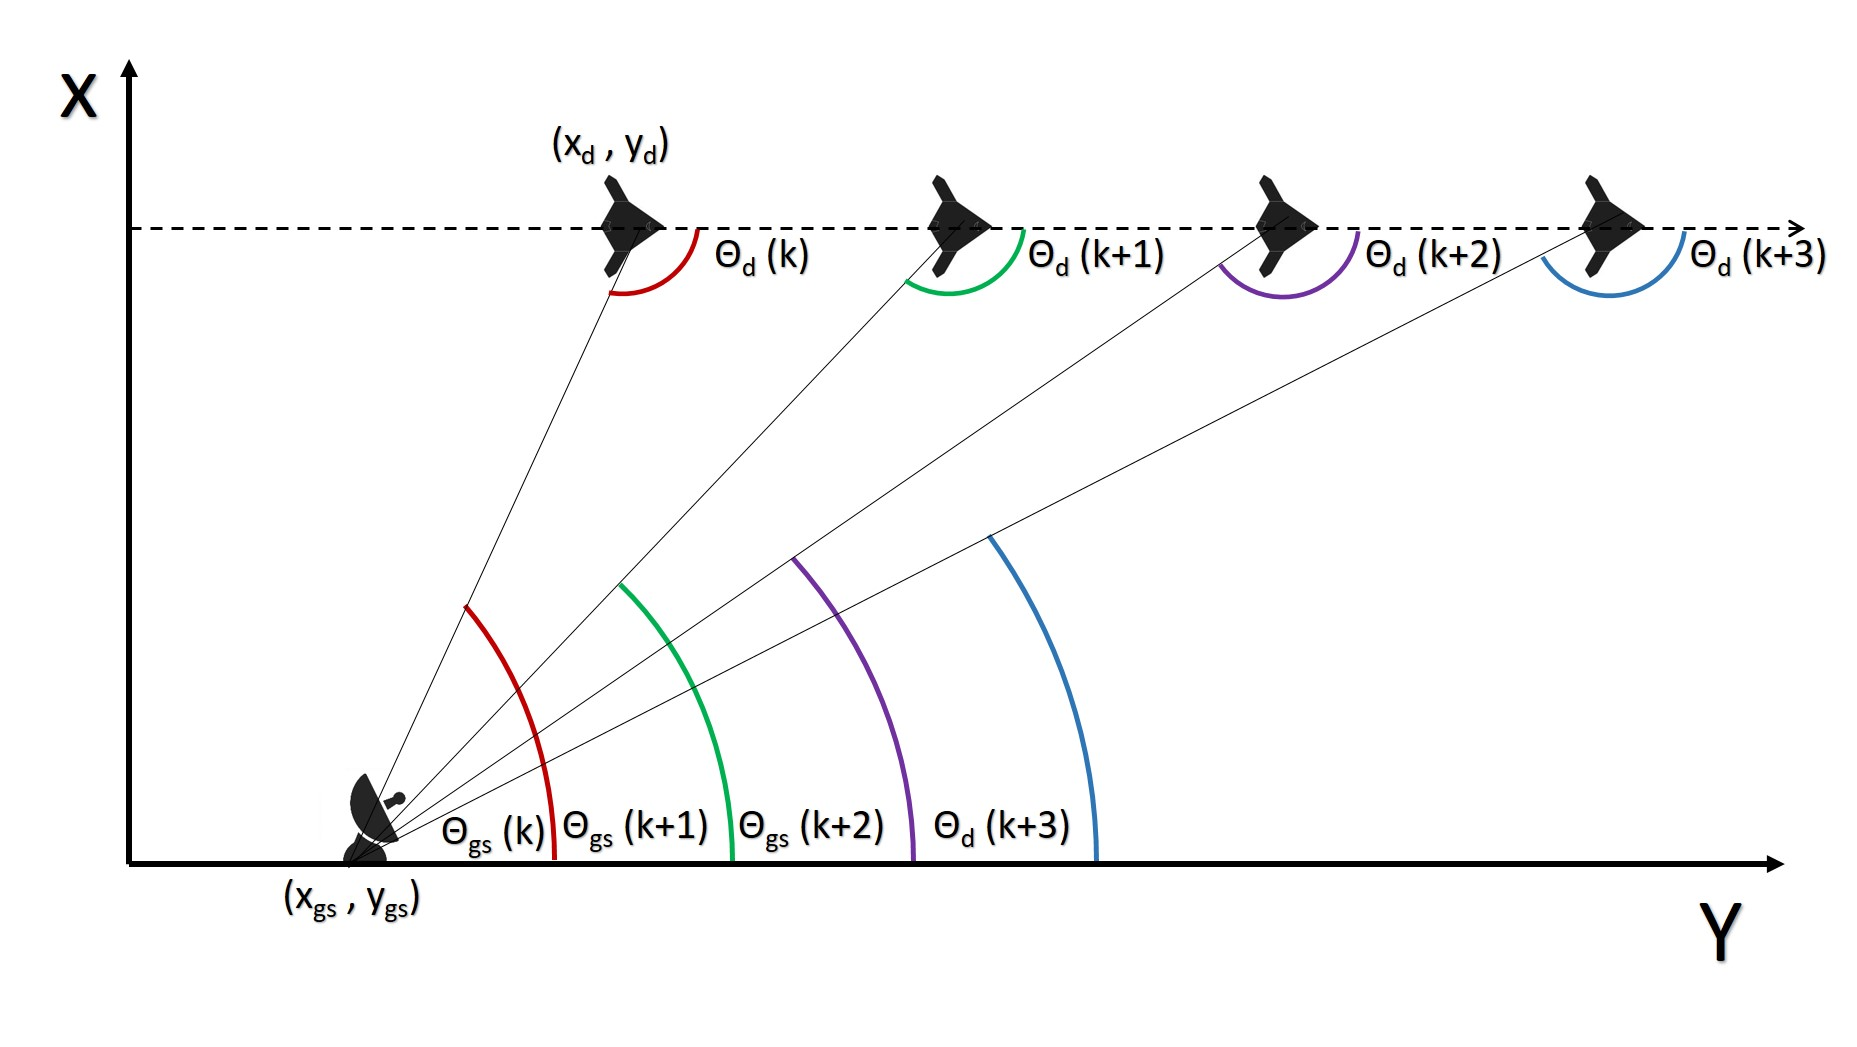
\includegraphics[scale=0.45]{figures/drone_gs_ex.jpg}
	\caption{Example of a drone-gs scenario}
	\label{fig:drone_gs}
\end{figure}

